% Options for packages loaded elsewhere
\PassOptionsToPackage{unicode}{hyperref}
\PassOptionsToPackage{hyphens}{url}
\PassOptionsToPackage{dvipsnames,svgnames,x11names}{xcolor}
%
\documentclass[
  letterpaper,
  DIV=11,
  numbers=noendperiod]{scrreprt}

\usepackage{amsmath,amssymb}
\usepackage{iftex}
\ifPDFTeX
  \usepackage[T1]{fontenc}
  \usepackage[utf8]{inputenc}
  \usepackage{textcomp} % provide euro and other symbols
\else % if luatex or xetex
  \usepackage{unicode-math}
  \defaultfontfeatures{Scale=MatchLowercase}
  \defaultfontfeatures[\rmfamily]{Ligatures=TeX,Scale=1}
\fi
\usepackage{lmodern}
\ifPDFTeX\else  
    % xetex/luatex font selection
\fi
% Use upquote if available, for straight quotes in verbatim environments
\IfFileExists{upquote.sty}{\usepackage{upquote}}{}
\IfFileExists{microtype.sty}{% use microtype if available
  \usepackage[]{microtype}
  \UseMicrotypeSet[protrusion]{basicmath} % disable protrusion for tt fonts
}{}
\makeatletter
\@ifundefined{KOMAClassName}{% if non-KOMA class
  \IfFileExists{parskip.sty}{%
    \usepackage{parskip}
  }{% else
    \setlength{\parindent}{0pt}
    \setlength{\parskip}{6pt plus 2pt minus 1pt}}
}{% if KOMA class
  \KOMAoptions{parskip=half}}
\makeatother
\usepackage{xcolor}
\setlength{\emergencystretch}{3em} % prevent overfull lines
\setcounter{secnumdepth}{5}
% Make \paragraph and \subparagraph free-standing
\makeatletter
\ifx\paragraph\undefined\else
  \let\oldparagraph\paragraph
  \renewcommand{\paragraph}{
    \@ifstar
      \xxxParagraphStar
      \xxxParagraphNoStar
  }
  \newcommand{\xxxParagraphStar}[1]{\oldparagraph*{#1}\mbox{}}
  \newcommand{\xxxParagraphNoStar}[1]{\oldparagraph{#1}\mbox{}}
\fi
\ifx\subparagraph\undefined\else
  \let\oldsubparagraph\subparagraph
  \renewcommand{\subparagraph}{
    \@ifstar
      \xxxSubParagraphStar
      \xxxSubParagraphNoStar
  }
  \newcommand{\xxxSubParagraphStar}[1]{\oldsubparagraph*{#1}\mbox{}}
  \newcommand{\xxxSubParagraphNoStar}[1]{\oldsubparagraph{#1}\mbox{}}
\fi
\makeatother

\usepackage{color}
\usepackage{fancyvrb}
\newcommand{\VerbBar}{|}
\newcommand{\VERB}{\Verb[commandchars=\\\{\}]}
\DefineVerbatimEnvironment{Highlighting}{Verbatim}{commandchars=\\\{\}}
% Add ',fontsize=\small' for more characters per line
\usepackage{framed}
\definecolor{shadecolor}{RGB}{241,243,245}
\newenvironment{Shaded}{\begin{snugshade}}{\end{snugshade}}
\newcommand{\AlertTok}[1]{\textcolor[rgb]{0.68,0.00,0.00}{#1}}
\newcommand{\AnnotationTok}[1]{\textcolor[rgb]{0.37,0.37,0.37}{#1}}
\newcommand{\AttributeTok}[1]{\textcolor[rgb]{0.40,0.45,0.13}{#1}}
\newcommand{\BaseNTok}[1]{\textcolor[rgb]{0.68,0.00,0.00}{#1}}
\newcommand{\BuiltInTok}[1]{\textcolor[rgb]{0.00,0.23,0.31}{#1}}
\newcommand{\CharTok}[1]{\textcolor[rgb]{0.13,0.47,0.30}{#1}}
\newcommand{\CommentTok}[1]{\textcolor[rgb]{0.37,0.37,0.37}{#1}}
\newcommand{\CommentVarTok}[1]{\textcolor[rgb]{0.37,0.37,0.37}{\textit{#1}}}
\newcommand{\ConstantTok}[1]{\textcolor[rgb]{0.56,0.35,0.01}{#1}}
\newcommand{\ControlFlowTok}[1]{\textcolor[rgb]{0.00,0.23,0.31}{\textbf{#1}}}
\newcommand{\DataTypeTok}[1]{\textcolor[rgb]{0.68,0.00,0.00}{#1}}
\newcommand{\DecValTok}[1]{\textcolor[rgb]{0.68,0.00,0.00}{#1}}
\newcommand{\DocumentationTok}[1]{\textcolor[rgb]{0.37,0.37,0.37}{\textit{#1}}}
\newcommand{\ErrorTok}[1]{\textcolor[rgb]{0.68,0.00,0.00}{#1}}
\newcommand{\ExtensionTok}[1]{\textcolor[rgb]{0.00,0.23,0.31}{#1}}
\newcommand{\FloatTok}[1]{\textcolor[rgb]{0.68,0.00,0.00}{#1}}
\newcommand{\FunctionTok}[1]{\textcolor[rgb]{0.28,0.35,0.67}{#1}}
\newcommand{\ImportTok}[1]{\textcolor[rgb]{0.00,0.46,0.62}{#1}}
\newcommand{\InformationTok}[1]{\textcolor[rgb]{0.37,0.37,0.37}{#1}}
\newcommand{\KeywordTok}[1]{\textcolor[rgb]{0.00,0.23,0.31}{\textbf{#1}}}
\newcommand{\NormalTok}[1]{\textcolor[rgb]{0.00,0.23,0.31}{#1}}
\newcommand{\OperatorTok}[1]{\textcolor[rgb]{0.37,0.37,0.37}{#1}}
\newcommand{\OtherTok}[1]{\textcolor[rgb]{0.00,0.23,0.31}{#1}}
\newcommand{\PreprocessorTok}[1]{\textcolor[rgb]{0.68,0.00,0.00}{#1}}
\newcommand{\RegionMarkerTok}[1]{\textcolor[rgb]{0.00,0.23,0.31}{#1}}
\newcommand{\SpecialCharTok}[1]{\textcolor[rgb]{0.37,0.37,0.37}{#1}}
\newcommand{\SpecialStringTok}[1]{\textcolor[rgb]{0.13,0.47,0.30}{#1}}
\newcommand{\StringTok}[1]{\textcolor[rgb]{0.13,0.47,0.30}{#1}}
\newcommand{\VariableTok}[1]{\textcolor[rgb]{0.07,0.07,0.07}{#1}}
\newcommand{\VerbatimStringTok}[1]{\textcolor[rgb]{0.13,0.47,0.30}{#1}}
\newcommand{\WarningTok}[1]{\textcolor[rgb]{0.37,0.37,0.37}{\textit{#1}}}

\providecommand{\tightlist}{%
  \setlength{\itemsep}{0pt}\setlength{\parskip}{0pt}}\usepackage{longtable,booktabs,array}
\usepackage{calc} % for calculating minipage widths
% Correct order of tables after \paragraph or \subparagraph
\usepackage{etoolbox}
\makeatletter
\patchcmd\longtable{\par}{\if@noskipsec\mbox{}\fi\par}{}{}
\makeatother
% Allow footnotes in longtable head/foot
\IfFileExists{footnotehyper.sty}{\usepackage{footnotehyper}}{\usepackage{footnote}}
\makesavenoteenv{longtable}
\usepackage{graphicx}
\makeatletter
\def\maxwidth{\ifdim\Gin@nat@width>\linewidth\linewidth\else\Gin@nat@width\fi}
\def\maxheight{\ifdim\Gin@nat@height>\textheight\textheight\else\Gin@nat@height\fi}
\makeatother
% Scale images if necessary, so that they will not overflow the page
% margins by default, and it is still possible to overwrite the defaults
% using explicit options in \includegraphics[width, height, ...]{}
\setkeys{Gin}{width=\maxwidth,height=\maxheight,keepaspectratio}
% Set default figure placement to htbp
\makeatletter
\def\fps@figure{htbp}
\makeatother
% definitions for citeproc citations
\NewDocumentCommand\citeproctext{}{}
\NewDocumentCommand\citeproc{mm}{%
  \begingroup\def\citeproctext{#2}\cite{#1}\endgroup}
\makeatletter
 % allow citations to break across lines
 \let\@cite@ofmt\@firstofone
 % avoid brackets around text for \cite:
 \def\@biblabel#1{}
 \def\@cite#1#2{{#1\if@tempswa , #2\fi}}
\makeatother
\newlength{\cslhangindent}
\setlength{\cslhangindent}{1.5em}
\newlength{\csllabelwidth}
\setlength{\csllabelwidth}{3em}
\newenvironment{CSLReferences}[2] % #1 hanging-indent, #2 entry-spacing
 {\begin{list}{}{%
  \setlength{\itemindent}{0pt}
  \setlength{\leftmargin}{0pt}
  \setlength{\parsep}{0pt}
  % turn on hanging indent if param 1 is 1
  \ifodd #1
   \setlength{\leftmargin}{\cslhangindent}
   \setlength{\itemindent}{-1\cslhangindent}
  \fi
  % set entry spacing
  \setlength{\itemsep}{#2\baselineskip}}}
 {\end{list}}
\usepackage{calc}
\newcommand{\CSLBlock}[1]{\hfill\break\parbox[t]{\linewidth}{\strut\ignorespaces#1\strut}}
\newcommand{\CSLLeftMargin}[1]{\parbox[t]{\csllabelwidth}{\strut#1\strut}}
\newcommand{\CSLRightInline}[1]{\parbox[t]{\linewidth - \csllabelwidth}{\strut#1\strut}}
\newcommand{\CSLIndent}[1]{\hspace{\cslhangindent}#1}

\KOMAoption{captions}{tableheading}
\makeatletter
\@ifpackageloaded{tcolorbox}{}{\usepackage[skins,breakable]{tcolorbox}}
\@ifpackageloaded{fontawesome5}{}{\usepackage{fontawesome5}}
\definecolor{quarto-callout-color}{HTML}{909090}
\definecolor{quarto-callout-note-color}{HTML}{0758E5}
\definecolor{quarto-callout-important-color}{HTML}{CC1914}
\definecolor{quarto-callout-warning-color}{HTML}{EB9113}
\definecolor{quarto-callout-tip-color}{HTML}{00A047}
\definecolor{quarto-callout-caution-color}{HTML}{FC5300}
\definecolor{quarto-callout-color-frame}{HTML}{acacac}
\definecolor{quarto-callout-note-color-frame}{HTML}{4582ec}
\definecolor{quarto-callout-important-color-frame}{HTML}{d9534f}
\definecolor{quarto-callout-warning-color-frame}{HTML}{f0ad4e}
\definecolor{quarto-callout-tip-color-frame}{HTML}{02b875}
\definecolor{quarto-callout-caution-color-frame}{HTML}{fd7e14}
\makeatother
\makeatletter
\@ifpackageloaded{bookmark}{}{\usepackage{bookmark}}
\makeatother
\makeatletter
\@ifpackageloaded{caption}{}{\usepackage{caption}}
\AtBeginDocument{%
\ifdefined\contentsname
  \renewcommand*\contentsname{Table of contents}
\else
  \newcommand\contentsname{Table of contents}
\fi
\ifdefined\listfigurename
  \renewcommand*\listfigurename{List of Figures}
\else
  \newcommand\listfigurename{List of Figures}
\fi
\ifdefined\listtablename
  \renewcommand*\listtablename{List of Tables}
\else
  \newcommand\listtablename{List of Tables}
\fi
\ifdefined\figurename
  \renewcommand*\figurename{Figure}
\else
  \newcommand\figurename{Figure}
\fi
\ifdefined\tablename
  \renewcommand*\tablename{Table}
\else
  \newcommand\tablename{Table}
\fi
}
\@ifpackageloaded{float}{}{\usepackage{float}}
\floatstyle{ruled}
\@ifundefined{c@chapter}{\newfloat{codelisting}{h}{lop}}{\newfloat{codelisting}{h}{lop}[chapter]}
\floatname{codelisting}{Listing}
\newcommand*\listoflistings{\listof{codelisting}{List of Listings}}
\usepackage{amsthm}
\theoremstyle{remark}
\AtBeginDocument{\renewcommand*{\proofname}{Proof}}
\newtheorem*{remark}{Remark}
\newtheorem*{solution}{Solution}
\newtheorem{refremark}{Remark}[chapter]
\newtheorem{refsolution}{Solution}[chapter]
\makeatother
\makeatletter
\makeatother
\makeatletter
\@ifpackageloaded{caption}{}{\usepackage{caption}}
\@ifpackageloaded{subcaption}{}{\usepackage{subcaption}}
\makeatother

\ifLuaTeX
  \usepackage{selnolig}  % disable illegal ligatures
\fi
\usepackage{bookmark}

\IfFileExists{xurl.sty}{\usepackage{xurl}}{} % add URL line breaks if available
\urlstyle{same} % disable monospaced font for URLs
\hypersetup{
  pdftitle={The Health Informaticist},
  pdfauthor={Hants Williams},
  colorlinks=true,
  linkcolor={blue},
  filecolor={Maroon},
  citecolor={Blue},
  urlcolor={Blue},
  pdfcreator={LaTeX via pandoc}}


\title{The Health Informaticist}
\author{Hants Williams}
\date{2024-10-28}

\begin{document}
\maketitle

\renewcommand*\contentsname{Table of contents}
{
\hypersetup{linkcolor=}
\setcounter{tocdepth}{2}
\tableofcontents
}

\bookmarksetup{startatroot}

\chapter*{Preface}\label{preface}
\addcontentsline{toc}{chapter}{Preface}

\markboth{Preface}{Preface}

\section*{Why?}\label{why}
\addcontentsline{toc}{section}{Why?}

\markright{Why?}

I started off, and still identify as a nurse, but now find myself
somewhere between the interaction of clinician and technologist. My job
as a professor involves teaching, and constantly aquiring new knowledge,
abilities, and skills (KSAs) between evidence based medicine (EBM) and
technology-focused tools that could be used to help us address these
issues. My curiosity and passion for BOTH healthcare and technology has
led me to pursue a variety of topics that I try to address in this book.
So what does this book cover?

This book covers python, healthcare data, medical codexes, open source
datasets, databases, cloud technologies, inferential statistics and
machine learning, visualizations, and related technologies important to
understand as a modern (future) health informaticsts.

I've created this book as the most important topics to me, and what I
have experienced within academic medical hospital systems, private
hospitals, consulting, and health tech-startups. So whether you're a
healthcare professional, data scientist, student, or enthusiast, this
book will offer you valuable insights and hopefully fun conversation and
dialgue related to what can be dry and boring material.

\subsubsection*{What You'll Find Here:}\label{what-youll-find-here}
\addcontentsline{toc}{subsubsection}{What You'll Find Here:}

\begin{itemize}
\tightlist
\item
  \textbf{A Broad Foundation}: Rather than in-depth on each topic, this
  book provides a wide overview, giving you a base to explore further.

  \begin{itemize}
  \tightlist
  \item
    An intro to\ldots{}\emph{Python}
  \item
    An intro to\ldots{}\emph{Healthcare Data}
  \item
    An intro to\ldots{}\emph{Inferential Statistics}
  \item
    An intro to\ldots{}\emph{Ai and Machine Learning}
  \item
    An intro to\ldots{}\emph{Supporting Cloud Technologies}
  \end{itemize}
\item
  \textbf{Hands-On Learning}: Chapters combine theory and practical
  examples, allowing you to apply what you learn through
  Pyodide-powered, interactive Python exercises.
\end{itemize}

\subsection*{Think Legos\ldots{}}\label{think-legos}
\addcontentsline{toc}{subsection}{Think Legos\ldots{}}

Think of each section as a component, or a lego, that when combined
together can lead to the creation of something useful. These core
technologies: databases, scripts, clouds, code languages, databases,
medical codexes\ldots etc that we will be exploring should be viewed as
individual lego pieces. It is our job as health informaticists to
understand which pieces exist, what they are capability of providing to
us, and then how we can put them together to make something unique and
useful. Key word is useful.

\begin{figure}[H]

{\centering 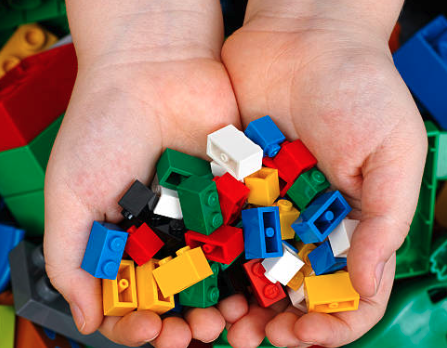
\includegraphics{lego.png}

}

\caption{Image of LEGO bricks as a metaphor for learning blocks}

\end{figure}%

\bookmarksetup{startatroot}

\chapter{Introduction}\label{introduction}

This is a book created from markdown and executable code.

See Knuth (1984) for additional discussion of literate programming.

\bookmarksetup{startatroot}

\chapter{Python Code - 1 - Hello
World}\label{python-code---1---hello-world}

\section{Objectives}\label{objectives}

The aim of this exercise is to learn how to write and execute Python
code.

\section{Rationale}\label{rationale}

There are plenty of
\href{https://en.wikipedia.org/wiki/List_of_programming_languages}{programing
languages}, but all of them share some common principles. Computers
execute \href{https://en.wikipedia.org/wiki/Machine_code}{machine code},
a binary set of instructions that are carried out by the computer
processors, but usually human do not write binary machine code, or even
\href{https://en.wikipedia.org/wiki/Assembly_language}{assembly
language}, the written code directly translatable to machine code.

Most of the time programers write code in languages that are easier to
write and read by us, humans. These codes, in turn, have to be
translated to machine code. This process of translation is called
\href{https://en.wikipedia.org/wiki/Compiler}{compilation}. Compilation
is a complex process that comprises several steps, and different
compilers and programming languages divide theses steps differently.
There are compilers, like the C or C++ compiles, that take the code and
compile it into a binary executable that can be directly run in a
computer, while there are other, like the Python
\href{https://en.wikipedia.org/wiki/Interpreter_(computing)}{interpreter}
of the Java compiler, that are capable of running directly the human
readable code that create an intermediate representation called
\href{https://en.wikipedia.org/wiki/Bytecode}{bytecode}. In these cases
we need to install the language interpreter to run the program. For
instance, if you want to run a Java or Python program you will need to
install Java or Python before.

\href{https://en.wikipedia.org/wiki/Python_(programming_language)}{Python}
is an interpreted language, so, once you install Python you will be able
to directly run Python code. However, you first need to have Python
available in your computer.

There are many ways of installing Python like:

\begin{itemize}
\tightlist
\item
  Downloading Python from \href{https://www.python.org/}{python.org}.
\item
  Using the Windows store or the Linux packages already prepared.
\item
  Using a Python version manager like
  \href{https://docs.astral.sh/uv/}{uv}.
\item
  Having Python included in your web browser thanks to
  \href{https://pyodide.org/}{Pyodide}.
\end{itemize}

In this exercise we are going to use
\href{https://pyodide.org/}{Pyodide}, a Python version that allow us to
run Python code directly in a web page without requiring any previous
installation.

The Notebook document is composed by cells, some are text (in markdown
format), and others contain Python code that can be executed. To execute
a Python cell:

\begin{itemize}
\tightlist
\item
  Select the cell that you want to execute.
\item
  Click the play symbol on top of the page or press shift + enter.
\end{itemize}

\section{Print Hello world}\label{print-hello-world}

\begin{Shaded}
\begin{Highlighting}[]
\NormalTok{\#| exercise: hello\_world\_01}
\NormalTok{print("Hello world")}
\end{Highlighting}
\end{Shaded}

\section{Print Hello ``Your Name''}\label{print-hello-your-name}

\begin{Shaded}
\begin{Highlighting}[]
\NormalTok{\#| exercise: hello\_world\_02}
\NormalTok{\# Use this Notebook cell to write Python code capable of printing your name}
\end{Highlighting}
\end{Shaded}

\begin{solution}
\leavevmode

\begin{tcolorbox}[enhanced jigsaw, opacityback=0, colframe=quarto-callout-tip-color-frame, breakable, colback=white, colbacktitle=quarto-callout-tip-color!10!white, titlerule=0mm, left=2mm, toprule=.15mm, coltitle=black, opacitybacktitle=0.6, bottomrule=.15mm, arc=.35mm, leftrule=.75mm, bottomtitle=1mm, toptitle=1mm, rightrule=.15mm, title=\textcolor{quarto-callout-tip-color}{\faLightbulb}\hspace{0.5em}{Tip}]

\begin{Shaded}
\begin{Highlighting}[]
\BuiltInTok{print}\NormalTok{(}\StringTok{\textquotesingle{}Jane\textquotesingle{}}\NormalTok{)}
\end{Highlighting}
\end{Shaded}

\end{tcolorbox}

\end{solution}

\bookmarksetup{startatroot}

\chapter{Python Code - 2 - Flow and
Variables}\label{python-code---2---flow-and-variables}

\section{Resources}\label{resources}

\begin{itemize}
\tightlist
\item
  \href{https://realpython.com/python-variables/}{Variables in Python}
  in Real Python.
\item
  \href{https://docs.python.org/3/library/functions.html\#print}{print}
  function official documentation.
\item
  A \href{https://realpython.com/python-print/}{print} function tutorial
  in Real Python.
\item
  \href{https://realpython.com/lessons/tuple-assignment-packing-unpacking/}{Variable
  unpaking} tutorial in Real Python.
\end{itemize}

\section{Flow}\label{flow}

The computer executes the programming code one line (or statement) at a
time. The order in which the lines are executed is called flow.

\begin{Shaded}
\begin{Highlighting}[]
\NormalTok{print("This line will be executed first.")}
\NormalTok{print("This line will be executed second.")}
\NormalTok{print("This line will be executed last.")}
\end{Highlighting}
\end{Shaded}

Order the lines in the following code, we want the computer to first say
Hello, then Your Name, and, finally, an invitation to play.

\begin{Shaded}
\begin{Highlighting}[]
\NormalTok{\#| exercise: fix\_flow}
\NormalTok{print("Your Name")}
\NormalTok{print("Do you want to play a nice game of chess?")}

\NormalTok{print("Hello")}
\end{Highlighting}
\end{Shaded}

\begin{tcolorbox}[enhanced jigsaw, opacityback=0, colframe=quarto-callout-note-color-frame, breakable, colback=white, colbacktitle=quarto-callout-note-color!10!white, titlerule=0mm, left=2mm, toprule=.15mm, coltitle=black, opacitybacktitle=0.6, bottomrule=.15mm, arc=.35mm, leftrule=.75mm, bottomtitle=1mm, toptitle=1mm, rightrule=.15mm, title=\textcolor{quarto-callout-note-color}{\faInfo}\hspace{0.5em}{Note}]

Remember that the lines are executed in order, so change the order of
the lines.

\end{tcolorbox}

\begin{solution}
\leavevmode

\begin{tcolorbox}[enhanced jigsaw, opacityback=0, colframe=quarto-callout-tip-color-frame, breakable, colback=white, colbacktitle=quarto-callout-tip-color!10!white, titlerule=0mm, left=2mm, toprule=.15mm, coltitle=black, opacitybacktitle=0.6, bottomrule=.15mm, arc=.35mm, leftrule=.75mm, bottomtitle=1mm, toptitle=1mm, rightrule=.15mm, title=\textcolor{quarto-callout-tip-color}{\faLightbulb}\hspace{0.5em}{Tip}]

\begin{Shaded}
\begin{Highlighting}[]
\BuiltInTok{print}\NormalTok{(}\StringTok{"Hello"}\NormalTok{)}
\BuiltInTok{print}\NormalTok{(}\StringTok{"John"}\NormalTok{)}
\BuiltInTok{print}\NormalTok{(}\StringTok{"Do you want to play a nice game of chess?"}\NormalTok{)}
\end{Highlighting}
\end{Shaded}

\end{tcolorbox}

\end{solution}

\section{Variables}\label{variables}

When we run programs we store information in the memory of the computer
for later use. This is a fundamental idea in computers. You can think
about the memory of a computer as a file cabinet in which we can store
values like numbers and strings of letters. Internally the memory is
divided in small pieces, like the drawers of a filing cabinet, and the
computer assings a numeric adress to each of those drawers. So, for
instance, we could tell the computer to store the number 42 in the
address 00000100, but it would be very cumbersome to use these numeric
addresses, so, instead, the we use
\href{https://en.wikipedia.org/wiki/Variable_(computer_science)}{variables},
names that we create, to refer to the memory locations and contents.

In different programming languages a variable can refer to the value
stored or to the memory address
(\href{https://en.wikipedia.org/wiki/Pointer_(computer_programming)}{pointer}).
In Python a variable will always be a reference to the object stored.
You can think of it as a label in the file cabinet drawer or an arrow
that points to the drawer.

\begin{figure}[H]

{\centering \includegraphics{../static/memory_and_variables.png}

}

\caption{Value stored in a variable}

\end{figure}%

In Python we store a variable in memory by using the assigment operator
\textbf{=}.

\begin{Shaded}
\begin{Highlighting}[]
\NormalTok{favorite\_number = 42}
\NormalTok{print("My favorite number is ", favorite\_number)}
\end{Highlighting}
\end{Shaded}

Python is doing quite a lot of things for us when we write
``favorite\_number = 42'':

\begin{enumerate}
\def\labelenumi{\arabic{enumi}.}
\tightlist
\item
  It reserves a space in the memory to be able to store the object that
  is going to create.
\item
  It creates the object 42.
\item
  It assigns the favorite\_number variable as a reference to the created
  and stored object.
\end{enumerate}

\section{Create and print variables}\label{create-and-print-variables}

Create two variables, one with your name, and another one with your
surname and print them.

\begin{Shaded}
\begin{Highlighting}[]
\NormalTok{\#| exercise: variable\_name}
\NormalTok{\# Fix this code, by providing a name and surname}

\NormalTok{name = }
\NormalTok{surname =}

\NormalTok{print("Hello ", name, " ", surname)}
\end{Highlighting}
\end{Shaded}

\begin{solution}
\leavevmode

\begin{tcolorbox}[enhanced jigsaw, opacityback=0, colframe=quarto-callout-tip-color-frame, breakable, colback=white, colbacktitle=quarto-callout-tip-color!10!white, titlerule=0mm, left=2mm, toprule=.15mm, coltitle=black, opacitybacktitle=0.6, bottomrule=.15mm, arc=.35mm, leftrule=.75mm, bottomtitle=1mm, toptitle=1mm, rightrule=.15mm, title=\textcolor{quarto-callout-tip-color}{\faLightbulb}\hspace{0.5em}{Tip}]

\begin{Shaded}
\begin{Highlighting}[]
\NormalTok{name = "Jane"}
\NormalTok{surname = "Doe"}
\NormalTok{print("Hello ", name, " ", surname)}
\end{Highlighting}
\end{Shaded}

\end{tcolorbox}

\end{solution}

Write the name and year of release of any movie using two variables.

\begin{Shaded}
\begin{Highlighting}[]
\NormalTok{\#| exercise: movie}
\NormalTok{\# write here the code to print the name and year of a movie}
\end{Highlighting}
\end{Shaded}

\begin{solution}
\leavevmode

\begin{tcolorbox}[enhanced jigsaw, opacityback=0, colframe=quarto-callout-tip-color-frame, breakable, colback=white, colbacktitle=quarto-callout-tip-color!10!white, titlerule=0mm, left=2mm, toprule=.15mm, coltitle=black, opacitybacktitle=0.6, bottomrule=.15mm, arc=.35mm, leftrule=.75mm, bottomtitle=1mm, toptitle=1mm, rightrule=.15mm, title=\textcolor{quarto-callout-tip-color}{\faLightbulb}\hspace{0.5em}{Tip}]

\begin{Shaded}
\begin{Highlighting}[]
\NormalTok{movie = "The Matrix"}
\NormalTok{year = 1999}
\NormalTok{print(movie, "was released in", year)}
\end{Highlighting}
\end{Shaded}

\end{tcolorbox}

\end{solution}

\section{Change the value of a
variable}\label{change-the-value-of-a-variable}

The variables can be changed to refer to different values/objects. Fix
the program to show your real name by changing the value of the
variable.

\begin{Shaded}
\begin{Highlighting}[]
\NormalTok{\#| exercise: variable\_change}
\NormalTok{name = "John"}
\NormalTok{name = }

\NormalTok{print("My name is ", name)}
\end{Highlighting}
\end{Shaded}

\begin{solution}
\leavevmode

\begin{tcolorbox}[enhanced jigsaw, opacityback=0, colframe=quarto-callout-tip-color-frame, breakable, colback=white, colbacktitle=quarto-callout-tip-color!10!white, titlerule=0mm, left=2mm, toprule=.15mm, coltitle=black, opacitybacktitle=0.6, bottomrule=.15mm, arc=.35mm, leftrule=.75mm, bottomtitle=1mm, toptitle=1mm, rightrule=.15mm, title=\textcolor{quarto-callout-tip-color}{\faLightbulb}\hspace{0.5em}{Tip}]

\begin{Shaded}
\begin{Highlighting}[]
\NormalTok{name = "John"}
\NormalTok{name = "Alice"}

\NormalTok{print("My name is ", name)}
\end{Highlighting}
\end{Shaded}

\end{tcolorbox}

\end{solution}

Given the following code, think about the expected output, what will the
program print when you execute it?

\begin{Shaded}
\begin{Highlighting}[]
\NormalTok{name = "FALKEN"}
\NormalTok{name = "SNAPE"}
\NormalTok{print(name)}
\NormalTok{name = "FALKEN"}
\NormalTok{print(name)}
\end{Highlighting}
\end{Shaded}

\section{Variables are not text
strings}\label{variables-are-not-text-strings}

Fix the following code to print the correct name of your Pokemons.

\begin{Shaded}
\begin{Highlighting}[]
\NormalTok{\#| exercise: variables\_and\_strings}
\NormalTok{my\_pokemon = "Pikachu"}
\NormalTok{your\_pokemon = "Ampharos"}
\NormalTok{print("My favorite pokemon is", "my\_pokemon")}
\NormalTok{print("Your favorite pokemon is", "your\_pokemon")}
\end{Highlighting}
\end{Shaded}

\begin{tcolorbox}[enhanced jigsaw, opacityback=0, colframe=quarto-callout-note-color-frame, breakable, colback=white, colbacktitle=quarto-callout-note-color!10!white, titlerule=0mm, left=2mm, toprule=.15mm, coltitle=black, opacitybacktitle=0.6, bottomrule=.15mm, arc=.35mm, leftrule=.75mm, bottomtitle=1mm, toptitle=1mm, rightrule=.15mm, title=\textcolor{quarto-callout-note-color}{\faInfo}\hspace{0.5em}{Note}]

Remember that variable names are not enclosed by quotes and that if you
put something inside a quote Python will consider it a text string.

\end{tcolorbox}

\begin{solution}
\leavevmode

\begin{tcolorbox}[enhanced jigsaw, opacityback=0, colframe=quarto-callout-tip-color-frame, breakable, colback=white, colbacktitle=quarto-callout-tip-color!10!white, titlerule=0mm, left=2mm, toprule=.15mm, coltitle=black, opacitybacktitle=0.6, bottomrule=.15mm, arc=.35mm, leftrule=.75mm, bottomtitle=1mm, toptitle=1mm, rightrule=.15mm, title=\textcolor{quarto-callout-tip-color}{\faLightbulb}\hspace{0.5em}{Tip}]

\begin{Shaded}
\begin{Highlighting}[]
\NormalTok{my\_pokemon = "Pikachu"}
\NormalTok{your\_pokemon = "Ampharos"}
\NormalTok{print("My favorite pokemon is", my\_pokemon)}
\NormalTok{print("Your favorite pokemon is", your\_pokemon)}
\end{Highlighting}
\end{Shaded}

\end{tcolorbox}

\end{solution}

It is very important to understand the difference between variables and
text:

\begin{itemize}
\tightlist
\item
  variable names are not enclosed by quotes.
\end{itemize}

\begin{Shaded}
\begin{Highlighting}[]
\NormalTok{a\_variable = 42}
\NormalTok{print("a\_variable")}
\NormalTok{print(a\_variable)}
\end{Highlighting}
\end{Shaded}

Fix the following code:

\begin{Shaded}
\begin{Highlighting}[]
\NormalTok{\#| exercise: fix\_variables}
\NormalTok{a = 4}
\NormalTok{b = 7}
\NormalTok{c = "a" + "b"}
\NormalTok{print("c is seven:", c)}
\end{Highlighting}
\end{Shaded}

\begin{solution}
\leavevmode

\begin{tcolorbox}[enhanced jigsaw, opacityback=0, colframe=quarto-callout-tip-color-frame, breakable, colback=white, colbacktitle=quarto-callout-tip-color!10!white, titlerule=0mm, left=2mm, toprule=.15mm, coltitle=black, opacitybacktitle=0.6, bottomrule=.15mm, arc=.35mm, leftrule=.75mm, bottomtitle=1mm, toptitle=1mm, rightrule=.15mm, title=\textcolor{quarto-callout-tip-color}{\faLightbulb}\hspace{0.5em}{Tip}]

\begin{Shaded}
\begin{Highlighting}[]
\NormalTok{a = 4}
\NormalTok{b = 7}
\NormalTok{c = a + b}
\NormalTok{print("c is seven:", c)}
\end{Highlighting}
\end{Shaded}

\end{tcolorbox}

\end{solution}

\section{Assignment unpaking}\label{assignment-unpaking}

Python allows for several variables to be set at the same time.

\begin{Shaded}
\begin{Highlighting}[]

\NormalTok{name, surname = "Ada", "Lovelace"}
\NormalTok{print(name, " ", surname, "was the first programmer")}

\NormalTok{temp1, temp2, temp3 = 36.5, 37.5, 39.5}
\NormalTok{print("The temperature has risen: ", temp1, " ", temp2, " ", temp3)}
\end{Highlighting}
\end{Shaded}

\bookmarksetup{startatroot}

\chapter{Python Code - 3 - Types}\label{python-code---3---types}

\section{Resources}\label{resources-1}

\begin{itemize}
\tightlist
\item
  Real Python tutorial:
  \href{https://realpython.com/python-data-types/}{basic data types}
\item
  Official documentation:
  \href{https://docs.python.org/3/library/stdtypes.html}{types and
  operations}.
\item
  Basic introduction to
  \href{https://github.com/JoseBlanca/py_industriales/blob/main/python/tipos_y_variables.ipynb}{type
  and variables},
  \href{https://github.com/JoseBlanca/py_industriales/blob/main/python/cadenas_de_texto.ipynb}{str}
  and
  \href{https://github.com/JoseBlanca/py_industriales/blob/main/python/booleanos.ipynb}{booleans}.
  (In Spanish).
\item
  \href{https://docs.python.org/3/library/functions.html\#type}{type}
  function official documentation.
\item
  Real Python introduction to
  \href{https://realpython.com/python-numbers/}{numbers} and
  \href{https://realpython.com/python-boolean/}{bool}.
\item
  A discussion about the
  \href{https://docs.python.org/3/tutorial/floatingpoint.html}{floating
  point arithmethic} in Python.
\end{itemize}

\section{Types}\label{types}

In a computer language variables have
\href{https://en.wikipedia.org/wiki/Data_type}{types}. For instance, we
have already used numbers and text strings.

\begin{Shaded}
\begin{Highlighting}[]
\NormalTok{\#| setup: true}
\NormalTok{\#| exercise: type01}

\NormalTok{\# this is to avoid a bug in quarto{-}live, that,}
\NormalTok{\# for some reason does not print the result of type}
\NormalTok{def type(obj):}
\NormalTok{    return obj.\_\_class\_\_.\_\_name\_\_}
\end{Highlighting}
\end{Shaded}

\begin{Shaded}
\begin{Highlighting}[]
\NormalTok{my\_number = 42}
\NormalTok{text = "My favorite number is"}
\NormalTok{print(text, my\_number)}
\end{Highlighting}
\end{Shaded}

We can ask for the type of variable (or object).

\begin{Shaded}
\begin{Highlighting}[]
\NormalTok{\#| exercise: type01}

\NormalTok{number = 42}
\NormalTok{print(\textquotesingle{}Type of the variable "number" is:\textquotesingle{}, type(number))}
\NormalTok{print(\textquotesingle{}Type of the string "42":\textquotesingle{}, type("42"))}
\end{Highlighting}
\end{Shaded}

The type for the number 42 is int and for the text string ``My favorite
number is'' is str. In most computer languages text is called string, or
something similar, because, for the computer, a text is a
\href{https://en.wikipedia.org/wiki/String_(computer_science)}{string of
characters}.

\section{Number types: int and float}\label{number-types-int-and-float}

In the previous example the type for the number was int
(\href{https://en.wikipedia.org/wiki/Integer_(computer_science)}{integer}),
but, in Python, and most other languages, we have another very important
numeric type: float
(\href{https://en.wikipedia.org/wiki/Floating-point_arithmetic}{floating
point number}).

\begin{Shaded}
\begin{Highlighting}[]
\NormalTok{\#| excercise: type02}

\NormalTok{integer = 42  \# type is int}
\NormalTok{floating\_point = 42.0  \# type is float}
\end{Highlighting}
\end{Shaded}

The main practical difference between the integer and float types is
that the arithmetic for integers will be exact, but for float will be
only approximate. This is not a Python quirk, but a general feature of
the computers.

\begin{Shaded}
\begin{Highlighting}[]
\NormalTok{number = 0.1 + 0.1 + 0.1 + 0.1 + 0.1 + 0.1 + 0.1 + 0.1 + 0.1 + 0.1}
\NormalTok{print(f\textquotesingle{}\{number:.50f\}\textquotesingle{})}
\end{Highlighting}
\end{Shaded}

Another practical limitation, besides the inherent error due to the
approximation, of the floating point arithmetic is that you have to be
careful when you compare floats.

\begin{Shaded}
\begin{Highlighting}[]
\NormalTok{first\_one = 0.1 + 0.1 + 0.1 + 0.1 + 0.1 + 0.1 + 0.1 + 0.1 + 0.1 + 0.1}
\NormalTok{second\_one = 1.0}
\NormalTok{print("Are first and second one the same number?", first\_one == second\_one)}

\NormalTok{\# But they are quite close}
\NormalTok{import math}
\NormalTok{print("Are first and second one close?", math.isclose(first\_one, second\_one))}

\NormalTok{\# with integers we don\textquotesingle{}t have this problem}
\NormalTok{first\_ten = 1 + 1 + 1 + 1 + 1 + 1 + 1 + 1 + 1 + 1}
\NormalTok{second\_ten = 10}
\NormalTok{print("Are first and second ten the same number?", first\_ten == second\_ten)}
\end{Highlighting}
\end{Shaded}

\section{Other types: bool and None}\label{other-types-bool-and-none}

bool (\href{https://en.wikipedia.org/wiki/Boolean_data_type}{boolean})
is a special type that can only have two values: True or False.

\begin{Shaded}
\begin{Highlighting}[]
\NormalTok{i\_am\_learning = True}
\NormalTok{print(type(i\_am\_learning), i\_am\_learning)}
\NormalTok{i\_am\_not\_here = False}
\NormalTok{print(type(i\_am\_not\_here), i\_am\_not\_here)}
\end{Highlighting}
\end{Shaded}

Another special type that you will find quite often in Python code is
None. This type can only have one value: None. It is usally employed
when you want to have a variable that still has no value, it signifies
that it is empty.

\begin{Shaded}
\begin{Highlighting}[]
\NormalTok{\#| setup: true}
\NormalTok{\#| exercise: type03}

\NormalTok{\# this is to avoid a bug in quarto{-}live, that,}
\NormalTok{\# for some reason does not print the result of type}
\NormalTok{def type(obj):}
\NormalTok{    return obj.\_\_class\_\_.\_\_name\_\_}
\end{Highlighting}
\end{Shaded}

\begin{Shaded}
\begin{Highlighting}[]
\NormalTok{\#| excercise: type03}
\NormalTok{result\_to\_be\_calculated = None}
\NormalTok{print(type(result\_to\_be\_calculated), result\_to\_be\_calculated)}
\NormalTok{\# Now we can calculate the result}
\NormalTok{result\_to\_be\_calculated = 42}
\NormalTok{print(result\_to\_be\_calculated)}
\end{Highlighting}
\end{Shaded}

\section{Python is dynamic}\label{python-is-dynamic}

In Python we don't need to specify the type of a variable before using
it, and we can even change the type of object that the variable refers
to. That is not the case in other languages, like C or Rust. In those
static languages the compiler needs to know the type of the variable
beforehand, and the type of a variable can not be changed.

\begin{Shaded}
\begin{Highlighting}[]
\NormalTok{\#| setup: true}
\NormalTok{\#| exercise: type04}

\NormalTok{\# this is to avoid a bug in quarto{-}live, that,}
\NormalTok{\# for some reason does not print the result of type}
\NormalTok{def type(obj):}
\NormalTok{    return obj.\_\_class\_\_.\_\_name\_\_}
\end{Highlighting}
\end{Shaded}

\begin{Shaded}
\begin{Highlighting}[]
\NormalTok{\#| exercise: type04}
\NormalTok{my\_number = None}
\NormalTok{print(type(my\_number), my\_number)}
\NormalTok{my\_number = 42}
\NormalTok{print(type(my\_number), my\_number)}
\NormalTok{my\_number = "42"}
\NormalTok{print(type(my\_number), my\_number)}
\NormalTok{my\_number = 42.0}
\NormalTok{print(type(my\_number), my\_number)}
\end{Highlighting}
\end{Shaded}

Modern Python has the option of specifying the types. This is not a
requirement, but you will see some
\href{https://docs.python.org/3/library/typing.html}{type hints} in
Python code.

\begin{Shaded}
\begin{Highlighting}[]
\NormalTok{my\_number: int = 42}
\NormalTok{my\_number: float = 42.0}
\NormalTok{my\_number: str = "42"}
\end{Highlighting}
\end{Shaded}

Be careful because Python does not enforce those type hints. If you
wanted to use them for anything else than documentation you would need a
type checker like \href{https://mypy-lang.org/}{mypy}. But if you are
starting in programming, just forget about this, the idea to remember is
that the objects refered to by the variables have types.

\section{Type casting}\label{type-casting}

\href{https://en.wikipedia.org/wiki/Type_conversion}{Type casting} or
type conversion is the action of changing one type into another. Python
has functions to do this type casting.

\begin{Shaded}
\begin{Highlighting}[]
\NormalTok{my\_number = 42}
\NormalTok{print(type(my\_number), my\_number)}
\NormalTok{my\_number = str(my\_number)}
\NormalTok{print(type(my\_number), my\_number)}
\NormalTok{my\_number = float(my\_number)}
\NormalTok{print(type(my\_number), my\_number)}
\NormalTok{my\_number = int(my\_number)}
\NormalTok{print(type(my\_number), my\_number)}
\end{Highlighting}
\end{Shaded}

We can also type cast to boolean.

\begin{Shaded}
\begin{Highlighting}[]
\NormalTok{print(bool(42))}
\NormalTok{print(bool(0))}
\NormalTok{print(bool("42"))}
\end{Highlighting}
\end{Shaded}

Find out which int and str values will be True and False when converted
to boolean.

\begin{Shaded}
\begin{Highlighting}[]
\NormalTok{\#| exercise: bool\_type\_casting}
\NormalTok{print(bool(value\_to\_test))}
\end{Highlighting}
\end{Shaded}

\begin{tcolorbox}[enhanced jigsaw, opacityback=0, colframe=quarto-callout-note-color-frame, breakable, colback=white, colbacktitle=quarto-callout-note-color!10!white, titlerule=0mm, left=2mm, toprule=.15mm, coltitle=black, opacitybacktitle=0.6, bottomrule=.15mm, arc=.35mm, leftrule=.75mm, bottomtitle=1mm, toptitle=1mm, rightrule=.15mm, title=\textcolor{quarto-callout-note-color}{\faInfo}\hspace{0.5em}{Note}]

Try with different int and str values, like 0, 1, 2, 3, ``Hello'', ''
``,''\,``.

\end{tcolorbox}

\begin{solution}
\leavevmode

\begin{tcolorbox}[enhanced jigsaw, opacityback=0, colframe=quarto-callout-tip-color-frame, breakable, colback=white, colbacktitle=quarto-callout-tip-color!10!white, titlerule=0mm, left=2mm, toprule=.15mm, coltitle=black, opacitybacktitle=0.6, bottomrule=.15mm, arc=.35mm, leftrule=.75mm, bottomtitle=1mm, toptitle=1mm, rightrule=.15mm, title=\textcolor{quarto-callout-tip-color}{\faLightbulb}\hspace{0.5em}{Tip}]

\begin{Shaded}
\begin{Highlighting}[]
\NormalTok{\# Any int, but 0, will be True}
\NormalTok{print("0", bool(0))}
\NormalTok{print("1", bool(0))}
\NormalTok{print("2", bool(2))}
\NormalTok{print("3", bool(3))}
\NormalTok{\# Any str, but the empty str, will be True}
\NormalTok{print(\textquotesingle{}""\textquotesingle{}, bool(""))}
\NormalTok{print(\textquotesingle{}"Hello"\textquotesingle{}, bool("Hello"))}
\NormalTok{print(\textquotesingle{}" "\textquotesingle{}, bool(" "))}
\end{Highlighting}
\end{Shaded}

\end{tcolorbox}

\end{solution}

Try to convert a boolean to integer.

\begin{Shaded}
\begin{Highlighting}[]
\NormalTok{\#| exercise: bool\_to\_int}

\NormalTok{\# what would be the result of converting the boolean values to integers?}
\end{Highlighting}
\end{Shaded}

\begin{solution}
\leavevmode

\begin{tcolorbox}[enhanced jigsaw, opacityback=0, colframe=quarto-callout-tip-color-frame, breakable, colback=white, colbacktitle=quarto-callout-tip-color!10!white, titlerule=0mm, left=2mm, toprule=.15mm, coltitle=black, opacitybacktitle=0.6, bottomrule=.15mm, arc=.35mm, leftrule=.75mm, bottomtitle=1mm, toptitle=1mm, rightrule=.15mm, title=\textcolor{quarto-callout-tip-color}{\faLightbulb}\hspace{0.5em}{Tip}]

\begin{Shaded}
\begin{Highlighting}[]
\NormalTok{print("True", int(True))}
\NormalTok{print("False", int(False))}
\end{Highlighting}
\end{Shaded}

\end{tcolorbox}

\end{solution}

\section{Why do we need types?}\label{why-do-we-need-types}

For a programming language using types is unavoidable. Different
languages have different types, but they all have types. Why? Because,
internally, the only thing that a computer can really stores in memory
is a binary number, and the same binary number can be interpreted as
different objects depending on its type.

\begin{Shaded}
\begin{Highlighting}[]
\NormalTok{print("The same binary number can represented an integer or a string, depending on its type")}
\NormalTok{binary\_number = 0b110100}
\NormalTok{print("The binary number is an integer that is usually printed in the decial number system:", binary\_number)}
\NormalTok{as\_a\_string = chr(binary\_number)}
\NormalTok{print("The binary number as a string:", as\_a\_string)}

\NormalTok{print("The number 4 as an integer and as a string be stored by the computer in different ways")}
\NormalTok{an\_object = 4}
\NormalTok{print(f"The binary representation for \{an\_object\} is: \{an\_object:b\}")}
\NormalTok{another\_object = "4"}
\NormalTok{print(f"The binary representation for \{another\_object\} is: \{ord(another\_object):b\}")}
\end{Highlighting}
\end{Shaded}

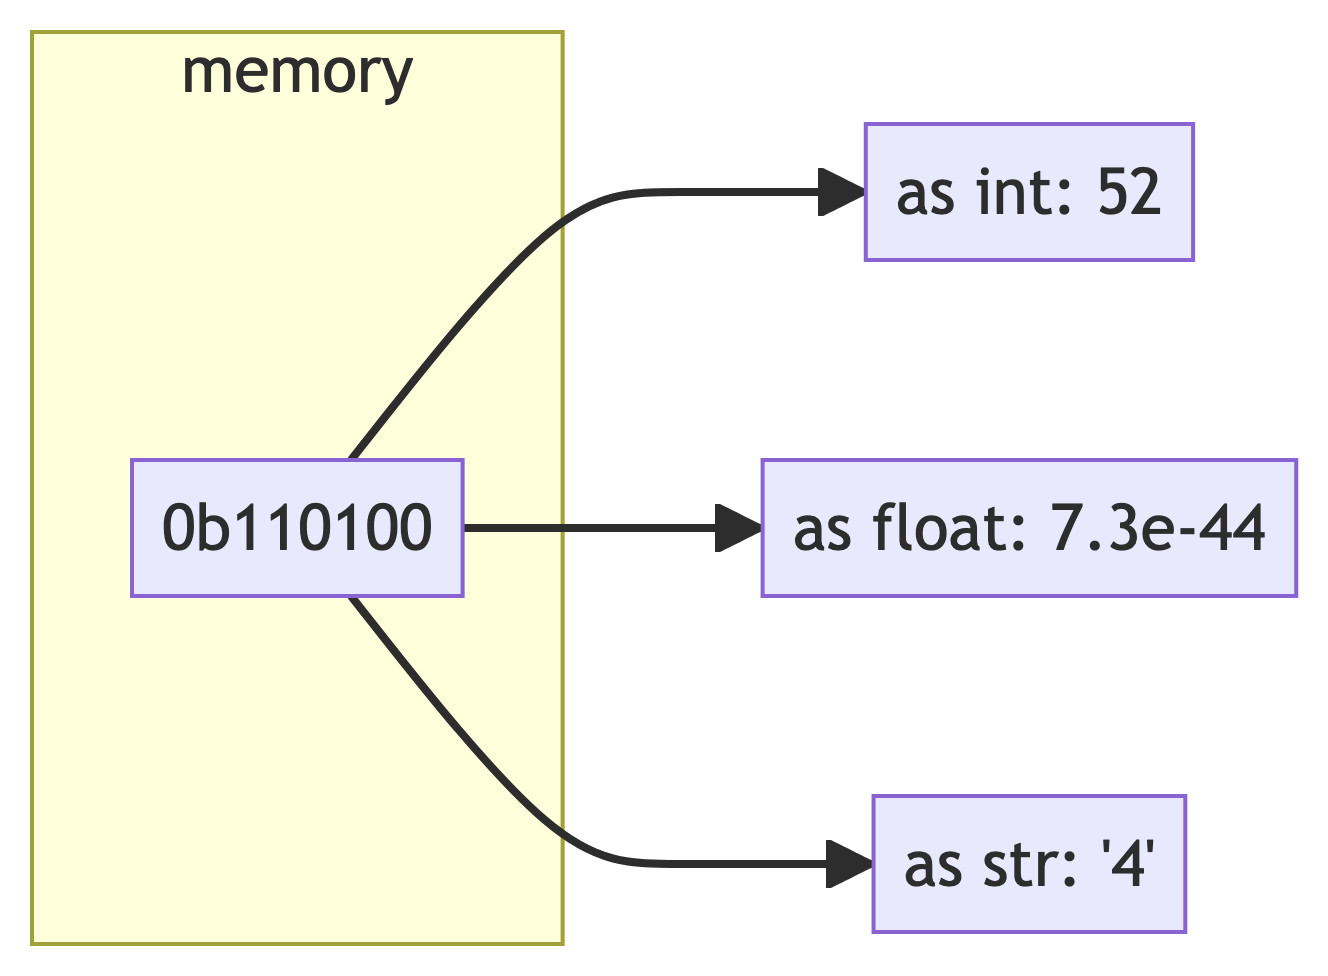
\includegraphics[width=3.46in,height=2.54in]{python_types_files/figure-latex/mermaid-figure-1.png}

\bookmarksetup{startatroot}

\chapter{Summary}\label{summary}

In summary, this book has no content whatsoever.

\bookmarksetup{startatroot}

\chapter*{References}\label{references}
\addcontentsline{toc}{chapter}{References}

\markboth{References}{References}

\phantomsection\label{refs}
\begin{CSLReferences}{1}{0}
\bibitem[\citeproctext]{ref-knuth84}
Knuth, Donald E. 1984. {``Literate Programming.''} \emph{Comput. J.} 27
(2): 97--111. \url{https://doi.org/10.1093/comjnl/27.2.97}.

\end{CSLReferences}




\end{document}
